\documentclass[tikz, border=10pt]{standalone}
%\documentclass[a4paper,12pt]{article}

\input{Preambulo.tex}
\input{Auxiliar.tex}

\begin{document}

\thispagestyle{empty}

    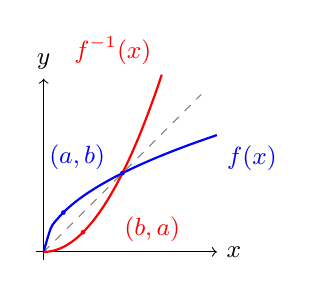
\begin{tikzpicture}
          % Eixos
          \draw[->] (-0.1,0) -- (2.2,0) node[right] {\small$x$};
          \draw[->] (0,-0.1) -- (0,2.2) node[above] {\small$y$};

          % Reta y = x (bissetriz)
          \draw[dashed, gray] (0,0) -- (2,2);

          % Função f (ex: f(x) = sqrt(x))
          \draw[domain=0:2.2, smooth, thick, blue] 
            plot (\x, {sqrt(\x)}) 
            node[below right] {\small$f(x)$};

          % Inversa f^{-1} (ex: f^{-1}(x) = x^2)
          \draw[domain=0:1.5, smooth, thick, red] 
            plot (\x, {\x*\x}) 
            node[above left] {\small$f^{-1}(x)$};

          % Pontos correspondentes
          \fill[blue] (1,1) circle[radius=0.03];
          \fill[blue] (0.25,0.5) circle[radius=0.03] node[xshift=5pt, yshift=20pt] {\small$(a,b)$};
          \fill[red] (0.5,0.25) circle[radius=0.03] node[xshift=25pt, yshift=1pt] {\small$(b,a)$};
          
        \end{tikzpicture}

\end{document}

#Como compilar e gerar uma imagem svg (Scalable Vector Graphics) para colocar em html
#pdflatex EsbocoTikz.tex
#pdf2svg EsbocoTikz.pdf EsbocoTikz.svg
